\documentclass[11pt]{article}

\usepackage{sectsty}
\usepackage{graphicx}
\usepackage{enumitem}
\usepackage{listings}
\usepackage{xcolor}
\usepackage{graphicx}
\usepackage{fancyhdr}

\definecolor{codegreen}{rgb}{0,0.6,0}
\definecolor{codegray}{rgb}{0.5,0.5,0.5}
\definecolor{codepurple}{rgb}{0.58,0,0.82}
\definecolor{backcolour}{rgb}{0.95,0.95,0.92}

\lstdefinestyle{mystyle}{
    backgroundcolor=\color{backcolour},   
    commentstyle=\color{codegreen},
    keywordstyle=\color{magenta},
    numberstyle=\tiny\color{codegray},
    stringstyle=\color{codepurple},
    basicstyle=\ttfamily\footnotesize,
    breakatwhitespace=false,         
    breaklines=true,                 
    captionpos=b,                    
    keepspaces=true,                 
    numbers=left,                    
    numbersep=5pt,                  
    showspaces=false,                
    showstringspaces=false,
    showtabs=false,                  
    tabsize=2
}

\lstset{style=mystyle}


% Margins
\topmargin=-0.45in
\evensidemargin=0in
\oddsidemargin=0in
\textwidth=6.5in
\textheight=9.0in
\headsep=0.25in

\title{ Web Technology\\ Assessment Solution\\2023 Fall \\ NCIT}

\author{ Sanjaya (Bir Bikram) Shrestha }
\date{\today}



\begin{document}
\maketitle	
\pagestyle{fancy}
\fancyhead[RO,LE]{\textbf{WT Solution 2021 Spring}}
\fancyfoot[RO,RE]{By: Sanjaya (Bir Bikram) Shrestha}

\tableofcontents
\pagebreak

% Optional TOC
% \tableofcontents
% \pagebreak

%--Paper--

\section{(Q No.1 A) To make an online presence or just transfer any data there are certain predefined rules to follow. Explain any 5 such commonly used protocols that serve different purposes of their own.}
\subparagraph{}

\begin{enumerate}
    \item \textbf{TCP/IP: (Transmission Control Protocol/Internet Protocol )} This is the foundation protocol of the internet and is used for communication between devices over the internet. The web browser sends a request to the website's server using the TCP/IP protocol and then server sends the requested web page back to the web browser using TCP/IP as well.

    \item \textbf{HTTP: (Hyper Text Transfer Protocol)} This is the protocol used for web browsing and transferring web pages from servers to clients. The browser sends http request to the server hosting the website. The server responds with an HTTP response, which includes the requested web page.
    
    \item \textbf{FTP: File transfer protocol} This is the protocol used for file transfer over the internet.  When we need to transfer a large file from one computer to another over the internet, you can use the FTP protocol. We need an FTP client program to connect to the FTP server where the file is stored, and then we can download the file using the FTP protocol.
    
    \item \textbf{SMTP: (Simple Mail Transfer Protocol)} This is the protocol used for email transmission between servers and clients. We are sending an email from your email client program to someone else's email address. Our email client uses the SMTP protocol to send the email to the email provider's SMTP server. The SMTP server then relays the email to the recipient's email provider using SMTP as well.
    
    \item \textbf{DNS: (Domain Name System)} This is the protocol used for translating domain names into IP addresses. When we type in a website URL into your web browser's address bar, the browser sends a request to a DNS server to look up the IP address associated with that URL. The DNS server responds with the IP address, which the web browser then uses to connect to the website's server.
    
    \item \textbf{SSH: (Secure Shell)} This is the protocol used for secure remote login and file transfer. If you need to remotely access a computer or server securely, you can use the SSH protocol. You'll need an SSH client program to connect to the remote computer or server, and then you can securely log in and transfer files using SSH.
    
    \item \textbf{DHCP: (Dynamic Host Control Protocol)} This is the protocol used for automatically assigning IP addresses to devices on a network. When a device joins a network, it can use DHCP to automatically obtain an IP address from the network's DHCP server. This allows devices to join a network without needing to manually configure IP addresses.
    
    \item \textbf{POP: (Post Office Protocol)} This is the protocol used for retrieving email from a server. We using an email client program like Microsoft Outlook or Apple Mail to download our email, we're likely using the POP protocol. POP allows email client to download all of your email from email provider's server and store it on local computer.
\end{enumerate}



\noindent\rule{\linewidth}{0.4pt}
\section{(Q No.1B) What happens when you enter https://ncit.edu.np into your browser? Describe along with its block diagram.}
\subparagraph{}
When we type https://ncit.edu.np into our  browser following steps will happen:
\begin{enumerate}
    \item Browser will initiates a request to the Domain Name System (DNS) to resolve the domain name "https://ncit.edu.np" into an IP address.
    \item The DNS responds with the IP address associated with the domain name, which in this case is the IP address of the server hosting the website.
    \item Browser will initiates a secure connection with the server using HTTPS protocol, which includes a series of handshaking and authentication steps to ensure the connection is secure and encrypted.
    \item The server responds with the HTML code for the home page of the pu.edu.np website.
    \item Browser then receives the HTML code and begins to parse it to render the page.
    \item The browser sends additional requests for any external files referenced in the HTML code, such as CSS stylesheets, images, and scripts.
    \item The server responds with the requested files and the browser uses them to render the page as intended.
    \item Then if we interact with the website, such as clicking a link or submitting a form, the browser sends additional requests to the server and the server responds with the appropriate content.
\end{enumerate}

\begin{lstlisting}
                            +---------------------+
                            | DNS Resolution      |
                            +---------------------+
                                        |
                                        v
    +------------+          +-----------------------+
    | Browser    |          | HTTPS Handshaking      |
    +------------+          +-----------------------+
            |                        |
            v                        v
    +-------------------+  +---------------------------+
    | Receive HTML code |  | Receive external resources |
    +-------------------+  +---------------------------+
            |                        |
            v                        v
    +-------------------+  +------------------------+
    | Parse HTML code   |  | Render page with assets |
    +-------------------+  +------------------------+
            |                        |
            v                        v
    +------------------+  +------------------+
    | Interact with website          |
    +------------------+  +------------------+

\end{lstlisting}

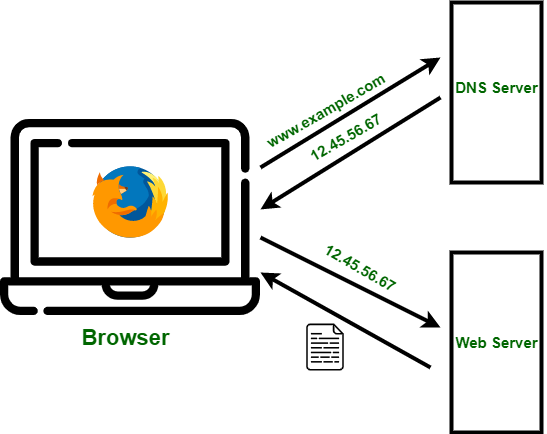
\includegraphics[width=0.5\textwidth]{resources/qno1b.png}

\noindent\rule{\linewidth}{0.4pt}
\section{(Q No.2A) Write HTML code for the following}
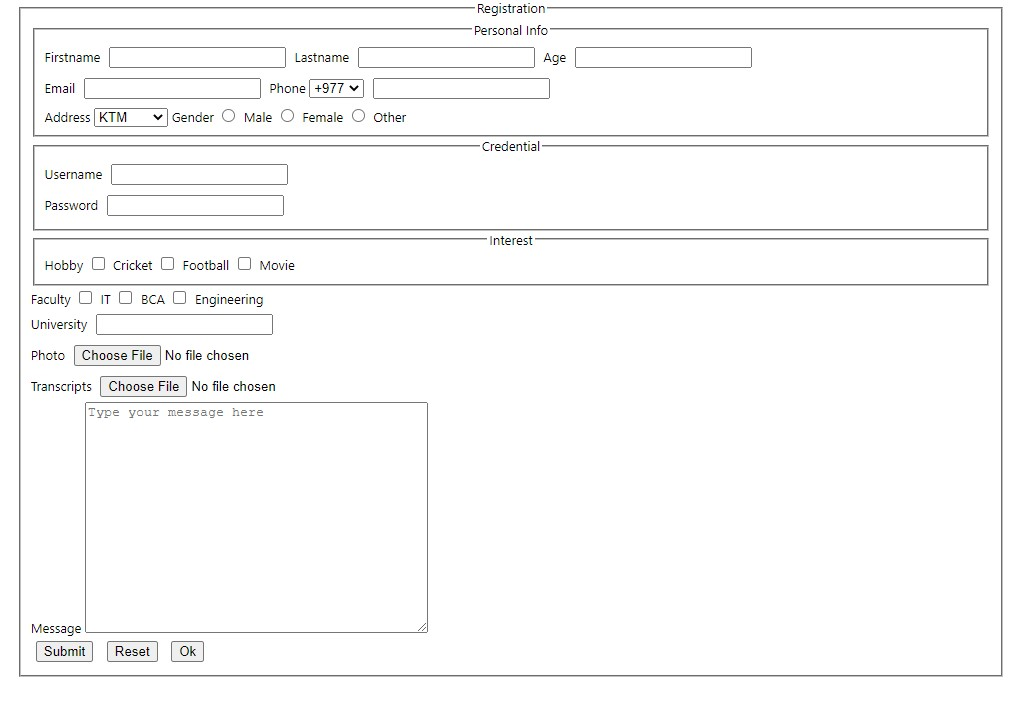
\includegraphics[width=0.75\textwidth]{resources/qno2a.jpg}
\subparagraph{}
\lstinputlisting[language=html]{resources/qno2a.html}




\noindent\rule{\linewidth}{0.4pt}
\section{(Q No.2B) How can you map images in HTML? Does a hyperlink apply to text only? Explain the logic behind it and its types in detail.}
\subparagraph{}
To map an image in HTML, you can use the $<$map$>$ and $<$area$>$ elements to define clickable regions on the image. Here's an example:
\begin{lstlisting}[language=html, caption={Image map}]
    <img src="https://fakeimg.pl/300/" alt="My Image" usemap="#myMap">

    <map name="myMap">
    <area shape="rect" coords="0,0,100,100" href="page1.html" alt="Page 1">
    <area shape="rect" coords="100,0,200,100" href="page2.html" alt="Page 2">
    <area shape="circle" coords="150,150,50" href="page3.html" alt="Page 3">
    </map>
\end{lstlisting}
When the user clicks on one of the mapped areas, the browser will navigate to the URL specified in the "href" attribute. This allows you to create interactive images that can act as navigation menus, image maps, and more.

No, hyperlinks in HTML do not apply to text only. We can create hyperlinks for any element that can have a clickable area, including images, buttons, and even entire divs.

A hyperlink is created using an <a> tag, which stands for "anchor." The $<$a$>$ tag requires a "href" attribute, which specifies the URL that the link should point to. We can also include text or other elements within the $<$a$>$ tag, which will serve as the clickable area for the hyperlink.

Here's an example of how to create a hyperlink for text in HTML:
\begin{lstlisting}[language=html]
    <a href="https://example.com">Click here to visit Example.com</a>
\end{lstlisting}

For email links also we can use the hyperlink. Email links are created using the mailto: protocol, like this:
\begin{lstlisting}[language=html]
    <a href="mailto:example@example.com">Send an email to Example</a>
\end{lstlisting}

For images we can use hyperlink like this:
\begin{lstlisting}[language=html]
    <a href="www.google.com"><img src="./google.png" alt="Click here to go to google"> </a>
\end{lstlisting}

Any clickable content inside the $<$a$>$ tag works for hyperlink.

\noindent\rule{\linewidth}{0.4pt}
\section{(Q No.3A) What are the overriding rule in CSS? Explain different levels of stylesheets with their hierarchy of implementation.}
\subparagraph{}
In CSS, the overriding rule is used to determine which style declarations should be applied to an element when there are multiple rules that could potentially apply.

The overriding rule in CSS can be summarized as follows:

\begin{enumerate}
    \item Styles defined using the !important keyword take precedence over all other styles, regardless of where they are defined in the CSS file.

    \item Styles defined inline (i.e. using the style attribute in an HTML element) take precedence over styles defined in an external CSS file or in the $<$head$>$ section of the HTML document.
    
    \item Styles defined closer to the element in the HTML document take precedence over styles defined further away. For example, styles defined in an ID selector take precedence over styles defined in a class selector, and styles defined in a class selector take precedence over styles defined in a tag selector.
    
    \item Styles defined with more specific selectors take precedence over styles defined with less specific selectors. For example, a style defined with a selector of \#my-div p (which targets all $<$p$>$ elements within an element with the ID of my-div) would take precedence over a style defined with a selector of p (which targets all $<$p$>$ elements on the page).
    
    \item Styles defined later in the CSS file take precedence over styles defined earlier in the file, provided that all other factors are equal.
\end{enumerate}
There are 3 levels of stylesheets in CSS:
\begin{enumerate}
    \item Inline Styles: These styles are applied directly to an HTML element using the style attribute. Inline styles have the highest specificity, meaning they override any other styles applied to the same element.
    \begin{lstlisting}[language=html, caption=Inline Style]
        <p style="color: red;">This text is red.</p>
    \end{lstlisting} 

    \item Internal Styles: These styles are defined within the head section of an HTML document using the style tag. Internal styles have a higher specificity than external styles, but lower than inline styles.
    \begin{lstlisting}[language=html, caption=Internal Style]

        <head>
    <style>
        p {
        color: blue;
        }
    </style>
    </head>
    <body>
    <p>This text is blue.</p>
    </body>
    \end{lstlisting} 
    
    \item External Styles: These styles are defined in an external CSS file and are linked to an HTML document using the link tag. External styles have the lowest specificity, but they are also the most reusable and easier to maintain.
    \begin{lstlisting}[language=html, caption=External Style]
    
            <head>
        <link rel="stylesheet" href="style.css">
        </head>
        <body>
        <p class="red-text">This text is red.</p>
        </body>
    \end{lstlisting} 
\end{enumerate}



\noindent\rule{\linewidth}{0.4pt}
\section{(Q No.3B) Design a box model. What will be the actual height and width of content if padding=margin=border=height=width of content = 20px?}
\subparagraph{}
The CSS box model is a container that contains multiple properties including borders, margin, padding, and the content itself. It is used to create the design and layout of web pages. It can be used as a toolkit for customizing the layout of different elements. The web browser renders every element as a rectangular box according to the CSS box model. Box-Model has multiple properties in CSS. \\
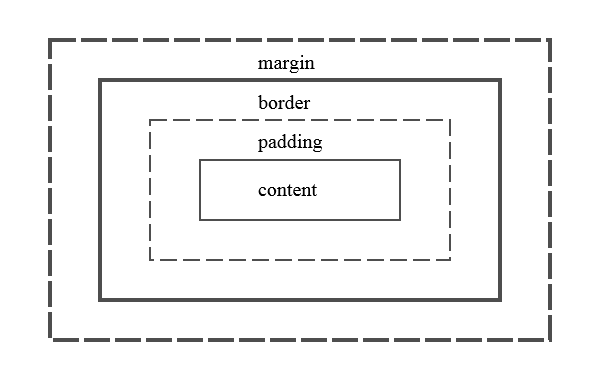
\includegraphics[width=0.75\textwidth]{resources/cssbox.png}

If the padding, margin, border, height, and width of an element's content are all set to 20 pixels, then the actual height and width of the content will be 0 pixels.

This is because the total size of the element would be calculated as follows:

Total size = height + padding + border + margin

Total size = 20px + 20px + 20px + 20px

Total size = 80px

Since the total size is greater than the height and width of the content (which are both set to 20 pixels), there is no space left over for the content itself. As a result, the content will be completely hidden and will not be visible on the page.



\noindent\rule{\linewidth}{0.4pt}
\section{(Q No.C) Write HTML and CSS code for the following O/P}
\subparagraph{}
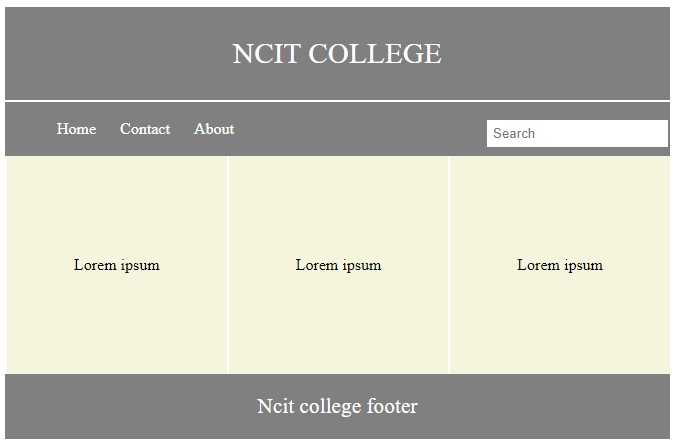
\includegraphics[width=0.75\textwidth]{resources/qno3c.jpg}

\lstinputlisting[language=html, caption={Html css for given design}]{resources/qno3c.html}


\noindent\rule{\linewidth}{0.4pt}
\section{(Q No.4A) How events are handled in JavaScript? Write the JS code for the following o/p. When the user provides quantity it gives total.}
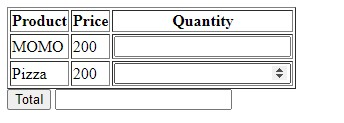
\includegraphics[width=0.75\textwidth]{resources/qno4a.jpg}
\subparagraph{}
In JavaScript, events are used to handle user interactions or system events, such as a mouse click or a keypress, and trigger corresponding actions.

To handle events in JavaScript, you can use event listeners. An event listener is a function that is executed in response to an event. Here's an example:
\begin{lstlisting}
    // Get a reference to the element you want to listen for an event on
const button = document.querySelector('button');

// Add an event listener to the element
button.addEventListener('click', function() {
  // Do something when the button is clicked
  alert("Hello World!!!");
});
In this example, we get a reference to a button element using document.querySelector(), and then add an event listener to it using the addEventListener() method. We pass in two arguments to addEventListener(): the type of event we want to listen for (in this case, 'click'), and the function we want to execute when the event occurs.

When the button is clicked, the function passed as the second argument to addEventListener() will be executed. Inside this function, we have alert function which will create a pop box when clicked.
\end{lstlisting}

Here is the JS code for the given scenario to display the total when quantity are given.
\lstinputlisting[language=html, caption={JS code to display total}]{resources/qno4a.html}

Here we have used onKeyUp function to handle the event, when key is pressed the event is triggered which will call the total() function in the JS, where we had created reference to the both quantity and price field, and then we checked if value is null then set to 0 for default value, then after converting to integer we calculated the total value then displaye in the total box.

\noindent\rule{\linewidth}{0.4pt}
\section{(Q No.4B) What do you  mean by DOM in JavaScript? Differences between DOM 0 and DOM 1 and DOM 2 methods with example.}
\subparagraph{}
In JavaScript, the DOM (Document Object Model) is an API that provides a way for JavaScript code to interact with HTML and XML documents as a tree of objects. The DOM represents the structure of a document as a tree of nodes and provides methods and properties for manipulating those nodes.

The differences between the DOM: DOM Level 0, DOM Level 1, and DOM Level 2 are:

\begin{itemize}
    \item DOM Level 0: This refers to the original, basic DOM API that was built into early versions of web browsers. It includes a few global objects and methods, such as document, window, and alert(), but doesn't provide a formalized API for working with the document tree. Instead, it allows directly manipulate the properties of the document and its elements using JavaScript.
    Example of using DOM Level 0:
    \begin{lstlisting}
        // Accessing the document object
        const doc = document;
    
        // Accessing an element and changing its text content
        const heading = document.getElementById('heading');
        heading.textContent = 'New Heading';
    \end{lstlisting}
    
    \item DOM Level 1: This introduced a formalized API for working with the document tree, including methods for accessing and manipulating elements and their attributes, as well as event handling. This version of the DOM is widely supported in modern browsers.
    Example of using DOM Level 1:
    \begin{lstlisting}
        // Accessing an element by ID and changing its text content
        const heading = document.getElementById('heading');
        heading.textContent = 'New Heading';
    
        // Adding an event listener to a button element
        const button = document.getElementById('myButton');
        button.addEventListener('click', function() {
        console.log('Button clicked!');
        });
    
    \end{lstlisting}
    
    \item DOM Level 2: This added additional features to the DOM, such as support for CSS styling and more advanced event handling. This version of the DOM is also widely supported in modern browsers.
    Example of using DOM Level 2:
    \begin{lstlisting}
        // Accessing an element's style properties
        const box = document.getElementById('myBox');
        box.style.backgroundColor = 'red';
        box.style.width = '100px';
        box.style.height = '100px';
    
        // Adding a mouseover event listener to an element
        const button = document.getElementById('myButton');
        button.addEventListener('mouseover', function() {
        this.style.backgroundColor = 'blue';
        });
    
    \end{lstlisting}
\end{itemize}


\noindent\rule{\linewidth}{0.4pt}
\section{(Q No.5A) Create a registration form as given. Also validates it with JavaScript. (All input should be fulfilled else *required message will display, the name must be of 8 characters, email should in the proper format. the phone must be of 10 digits, password include only number and must be of 8 digits, and starting and ending with 0, Confirm password and Password must match).}
\subparagraph{}



\noindent\rule{\linewidth}{0.4pt}
\section{(Q No.1 A) To make an online presence or just transfer any data there are certain predefined rules to follow. Explain any 5 such commonly used protocols that serve different purposes of their own.}
\subparagraph{}
\end{document}